\documentclass[pdf]{beamer}
\usetheme{metropolis}

\usepackage[utf8]{inputenc} % allow utf-8 input
\usepackage[T1]{fontenc}    % use 8-bit T1 fonts
\usepackage{hyperref}       % hyperlinks
\usepackage{url}            % simple URL typesetting
\usepackage{booktabs}       % professional-quality tables
\usepackage{amsfonts}       % blackboard math symbols
\usepackage{nicefrac}       % compact symbols for 1/2, etc.
\usepackage{microtype}      % microtypography
\usepackage{amsmath}        % math notation etc
\usepackage{graphicx}       % inserting images
\usepackage{float}          % image placement
\usepackage{array}          % table alignment
\usepackage{xcolor}         % to do macro
\usepackage{adjustbox}      % Shrink stuff

\newcommand{\R}{\mathbb{R}}
\newcommand{\E}{\mathbb{E}}
\newcommand{\bx}{\boldsymbol{x}}
\newcommand{\todo}[1]{\textcolor{red}{#1}}

\graphicspath{ {../figures/} }

\title{On Gaussian Processes for Regression}
\author{
  \textbf{Jeffrey Alido} \\
  Department of Electrical and Computer Engineering \\
  Boston University \\
  \texttt{jalido@bu.edu} \\
  \and \\
  \textbf{Shashank Manjunath} \\
  Department of Electrical and Computer Engineering \\
  Boston University \\
  \texttt{manjuns@bu.edu}
}
\date{April 27, 2021}

\begin{document}

\begin{frame}
  \titlepage
\end{frame}

\begin{frame}
  \frametitle{Introduction}

  \begin{itemize}
    \item Gaussian processes are a class of machine learning models that allow us to easily incorporate prior
      observations into our data. 
    \item Example: predicting temperatures throughout a room.
    \begin{itemize}
      \item Suppose you are trying to determine the temperature at a certain point in a room, $\bx_{n+1}$
      \item You know the temperatures at points $\{\bx_1, \hdots, \bx_n\}$
      \item If $\{\bx_1, \hdots, \bx_n, \bx_{n+1}\}$ are close, the temperatures at these points will be highly
        correlated
      \item If they are far apart, the temperatures will be less correlated.
      \item We can model the $n$ known points as a multivariate Gaussian distribution with the covariance of points
        $\bx_i$ and $\bx_j$ dependent on the physical distance between the two points, then use our distribution to
        predict the temperature at $\bx_{n+1}$
    \end{itemize}
  \end{itemize}
\end{frame}

\begin{frame}
  \frametitle{Introduction}
  \begin{itemize}
    \item In a GP, we assume any new points we observe follow the same multivariate normal observed in our training data
    \item Some history of GPs 
    	\cite{rasmussen_gaussian_2006}
    \begin{itemize}
      \item Blight and Ott first introducted GPs as priors over functions in 1975\cite{kuss_gaussian_2006}
      \item Gaussian Process models were first recognized as the limit of a Bayesian neural network by Mackay (1992) and
        Neal (1996)\cite{kuss_gaussian_2006}
    \end{itemize}
    \item GPs are non-parametric models (unlike models such as Neural Networks)\cite{bishop_pattern_2006}
    \item GPs allows us to quantify uncertainty in our predictions
    \item GPs are not advantageous in that they scale poorly to large datasets
  \end{itemize}
\end{frame}

\begin{frame}
  \frametitle{Multivariate Gaussian Distributions}

  \begin{itemize}
    \item A set of univariate Gaussian random variables may be characterized jointly as a multivariate Gaussian
      distribution, with joint probability distribution fully characterized by a mean vector and a covariance matrix:

      \[
        X = \begin{bmatrix}
                 X_{1} \\
                 X_{2} \\
                 \vdots \\
                 X_{n}
               \end{bmatrix}   \sim \mathcal{N}(\boldsymbol{\mu},\Sigma)
      \]
      \begin{itemize}
        \item $\boldsymbol{\mu} \in \R^{n}$ indicates the mean vector
        \item $\Sigma \in \R^{n \times n}$ indicates the covariance matrix whose entries describe the covariance between
          each pair of random variables
      \end{itemize}
  \end{itemize}
\end{frame}

\begin{frame}
  \frametitle{Gaussian Processes}
  \begin{itemize}
    \item A Gaussian process $f(\boldsymbol{x})$ is defined as a a random process where each set of random variable in
      the random process is has a multivariate Gaussian distribution.
    \item In mathematical notation, $f(\boldsymbol{x})$ is fully characterized by a mean function  $m(\boldsymbol{x})$
      and covariance function, $K(\boldsymbol{x},\boldsymbol{x'})$:
      \begin{gather*}
        f(\boldsymbol{x})\sim\mathcal{GP}(m(\boldsymbol{x}),K(\boldsymbol{x},\boldsymbol{x'})) \\
        K(\bx, \bx') = \E[(f(\bx) - m(\bx))(f(\bx') - m(\bx'))]
      \end{gather*}

    \item The mean function $m(\bx)$ is typically defined as zero
    \item The covariance is chosen based on some prior belief about the dataset
    \item The covariance function is analagous to a kernel function $\kappa(\cdot, \cdot)$, where each entry of the
      covariance matrix is the kernel function calculated between the corresponding points
  \end{itemize}
\end{frame}

\begin{frame}
  \frametitle{Gaussian Processes for Regression}

  \begin{itemize}
    \item While we have defined a Gaussian process, we now describe how to fit a Gaussian process (predictive
      distribution) given a training set (prior distribution) and test points
    \item Suppose we observe training data $\bx$, test data $\bx'$, and choose kernel $\kappa$. Then the mean and
      covariance functions are given by 

      \begin{gather*}
        m(\boldsymbol{x})=\kappa(\bx, \bx')^\top \left(\kappa(\bx, \bx) + \sigma_{n}^{2} I\right)^{-1}\bx \\
        K(\boldsymbol{x},\boldsymbol{x'}) = \kappa(\bx', \bx') - \kappa(\bx, \bx')^{\top}\left(\kappa(\bx, \bx) +
        \sigma_{n}^{2}I\right)^{-1}\kappa(\bx, \bx')
      \end{gather*}
  \end{itemize}

  Those interested in a full derivation of the results are encouraged to consult section 2 of
  \cite{rasmussen_gaussian_2006}.
\end{frame}

\begin{frame}
  \frametitle{Kernels}
  \begin{itemize}
    \item Gaussian processes use kernels to help project input features into alternate feature
      spaces\cite{duvenaud_automatic_2014}
      \begin{itemize}
        \item We test out 6 different kernels, and use 5-fold cross validation grid search to find the best
          hyperparameters
      \end{itemize}
    \item We can additionally combine simple kernels to create more complicated kernels
    \begin{itemize}
      \item We test out the Local Periodic Kernel, which is a combination of the Squared Exponential and Periodic
        kernels
    \end{itemize}
    \item Kernel choice is up to you - you know the problem best!
  \end{itemize}
\end{frame}

\begin{frame}
  \frametitle{A Simple Demonstration}
  \vspace*{-1cm}
  \hspace*{-2cm} 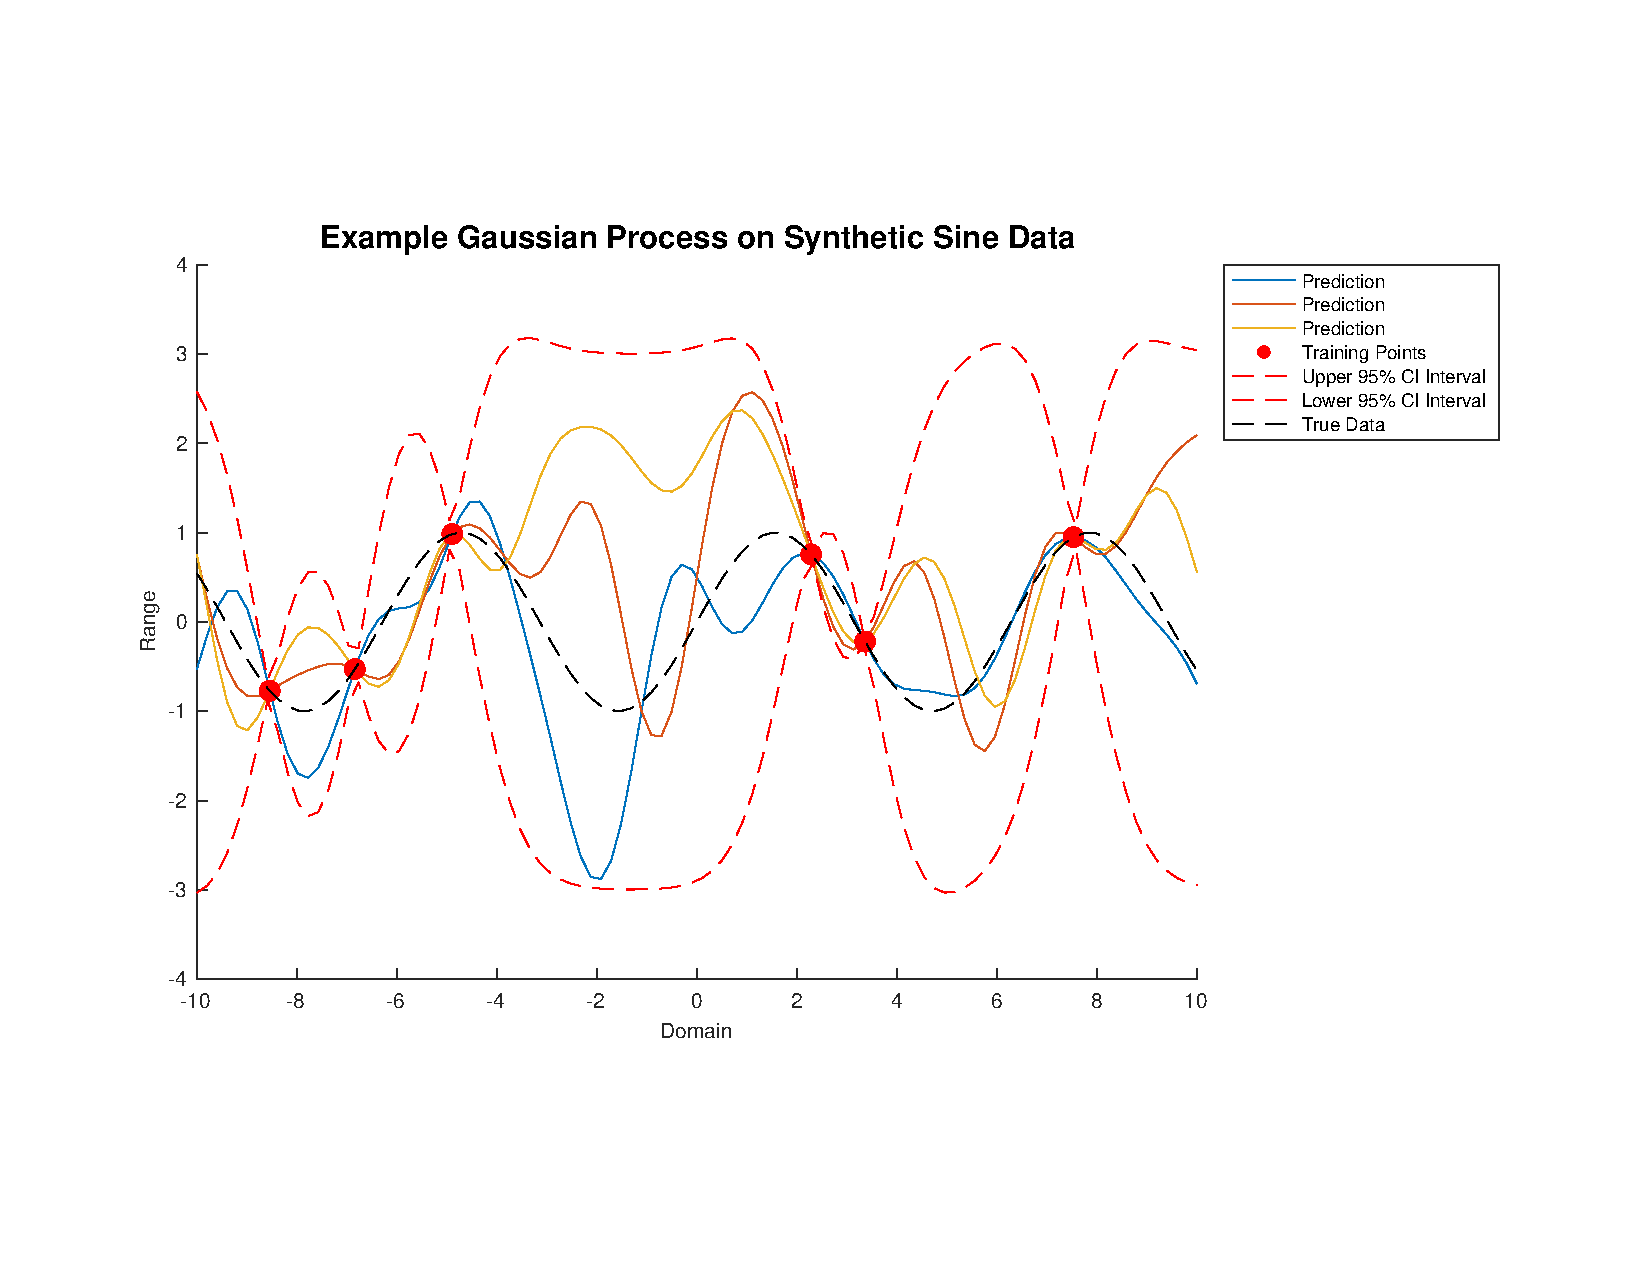
\includegraphics[scale=0.5]{synthetic_data}
\end{frame}

\begin{frame}
  \frametitle{The Boston Housing Dataset}
  \begin{itemize}
    \item Originally published in 1978\cite{harrison_hedonic_1978}
    \item 506 data points, 13 features, 1 label (median value of a house in a Boston suburb, in \$1000s)
    \item Well-suited to Gaussian processes due to small size
    \item Features detailed in Table \ref{table:bhd_feat}
  \end{itemize}
\end{frame}

\begin{frame}
  \begin{table}
    \centering
    \caption{Table of Boston Housing Dataset feature names and features}
    \resizebox{1.25\textheight}{!}{
      \begin{tabular}{ || m{3cm} | m{12cm} || }
        \hline
        \textbf{Feature Name} & \textbf{Feature Description} \\
        \hline \hline
        CRIM    & Per capita crime rate by town \\
        \hline
        ZN      & Proportion of residential land zoned for lots over 25,000 sq.ft. \\
        \hline
        INDUS   & Proportion of non-retail business acres per town. \\
        \hline
        CHAS    & Charles River dummy variable (1 if tract bounds river; 0 otherwise) \\
        \hline
        NOX     & Nitric oxides concentration (parts per 10 million) \\
        \hline
        RM      & Average number of rooms per dwelling \\
        \hline
        AGE     & Proportion of owner-occupied units built prior to 1940 \\
        \hline
        DIS     & Weighted distances to five Boston employment centres \\
        \hline
        RAD     & Index of accessibility to radial highways \\
        \hline
        TAX     & Full-value property-tax rate per \$10,000 \\
        \hline
        PTRATIO & Pupil-teacher ratio by town \\
        \hline
        B       & $1000(Bk - 0.63)^2$ where Bk is the proportion of Black people by town \\
        \hline
        LSTAT   & \% lower status of the population \\
        \hline
        MEDV    & Median value of owner-occupied homes in \$1000's \\
        \hline
      \end{tabular}
    }
    \label{table:bhd_feat}
  \end{table}
\end{frame}

\begin{frame}
  \frametitle{Implementation Details}

  \begin{itemize}
    \item We implemented grid search for our hyperparameters
    \item We normalize our features, which leads to improved algorithm performance, using the following
      formula:

      \[
        X_{\text{feat}} = \frac{X_{\text{feat}} - \mu(X_{\text{feat}})}{\sigma(X_{\text{feat}})}
      \]
    \item We also normalize our label, then convert back to given units (value in \$1000s) after fitting the GP.
    \item We use the RMSE metric:
      \[
        RMSE = \sqrt{\frac{\sum\limits_{i=1}^{N} (y_i - \hat y_i)^{2}}{N}}
      \]

      where $y_i$ is the true value, $\hat y_i$ is the predicted value, and $N$ is the number of samples

  \end{itemize}
\end{frame}

\begin{frame}
  \frametitle{Results}

  \begin{itemize}
    \item All values presented are RMSE values
    \item We present Regression SVM (trained with cross-validation hyperparameter search) test error values and Linear
      Regression test error values for comparison
    \item Linear Regression: \textbf{4.751}
  \end{itemize}

  \begin{table}
    \centering
    \caption{Table of Boston Housing Dataset feature names and features}
    \resizebox{\textheight}{!}{
      \begin{tabular}{ || m{3cm} | m{3cm} | m{3cm} | m{3cm} || }
        \hline
        & \textbf{Gaussian Process Regressor} & \textbf{SVM Regressor} & Linear Regression \\
        \hline
        Linear Kernel & \textbf{4.751} & 4.935 & \textbf{4.751} \\
        \hline
        Square Exp Kernel & \textbf{3.586} & 9.014 & 4.751 \\
        \hline
        Rational Quadratic Kernel & \textbf{3.560} & 9.013 & 4.751 \\
        \hline
        Periodic Kernel & 8.944 & 9.017 & \textbf{4.751} \\
        \hline
        Local Periodic Kernel & 5.065 & 9.014 & \textbf{4.751} \\
        \hline
        Polynomial Kernel & \textbf{4.213} & 80.389 & 4.751 \\
        \hline
      \end{tabular}
    }
  \end{table}
\end{frame}

\begin{frame}[shrink=30]
  \frametitle{References}
  % \bibliographystyle{amsalpha}
  \bibliographystyle{ieeetr}
  \bibliography{../gpr}

  Code for MATLAB implementation, LaTeX for presentation and paper can be found
  \href{https://github.com/shashankmanjunath/GaussianProcessRegression}{on Github at
  https://github.com/shashankmanjunath/GaussianProcessRegression}

\end{frame}
\end{document}
